\documentclass[aspectratio=169,11pt]{beamer}
\usepackage[utf8]{inputenc}
\usepackage{graphicx}
\usepackage{tikz}
\usetikzlibrary{arrows.meta,positioning}

\definecolor{Tinta}{HTML}{102C49}
\definecolor{Azul}{HTML}{205C94}
\definecolor{Claro}{HTML}{DEEAF5}
\definecolor{Fundo}{HTML}{F8FAFC}
\definecolor{Suave}{HTML}{536B80}
\setbeamercolor{normal text}{fg=Tinta,bg=Fundo}
\setbeamercolor{frametitle}{fg=Tinta,bg=Fundo}
\setbeamercolor{structure}{fg=Azul}
\setbeamercolor{bloco}{fg=Tinta,bg=Claro}
\setbeamercolor{rodape}{fg=Suave,bg=Fundo}
\setbeamerfont{frametitle}{size=\Large,series=\bfseries}
\setbeamersize{text margin left=9mm,text margin right=9mm}
\setbeamertemplate{navigation symbols}{}
\setbeamertemplate{itemize item}{\small\raisebox{.15ex}{$\bullet$}}
\setbeamertemplate{footline}{%
  \begin{beamercolorbox}[wd=\paperwidth,ht=4.8ex,dp=2ex,leftskip=9mm,rightskip=9mm]{rodape}%
    \raisebox{-1ex}{
\includegraphics[height=10ex]{figuras/lps.png}}\hfill\footnotesize\insertframenumber/\inserttotalframenumber
  \end{beamercolorbox}%
}
\newcommand{\mensagem}[1]{\vfill{\color{Azul}\bfseries #1}\par\smallskip}
\newcommand{\fonte}[1]{\par\smallskip{\footnotesize\color{Suave}#1}\par}
\newcommand{\painel}[2]{%
  \colorbox{Claro}{\parbox[c][19mm][c]{\dimexpr#1-2\fboxsep\relax}{\centering #2}}%
}
\newcommand{\comparar}[2]{%
  \begin{columns}[onlytextwidth,c]
    \column{.47\textwidth}\painel{\linewidth}{#1}
    \column{.47\textwidth}\painel{\linewidth}{#2}
  \end{columns}%
}
\tikzset{
  etapa/.style={fill=Claro,align=center,inner sep=3pt,minimum height=12mm},
  seta/.style={-{Latex[length=2mm]},thick,draw=Azul}
}
\title{Representation Learning}
\author{Vinícius Ferreira Neves}
\institute{CPE727 \ensuremath{\cdot} Aprendizado Profundo \ensuremath{\cdot} PEE/COPPE/UFRJ}
\date{}

\begin{document}

{
\setbeamercolor{background canvas}{bg=Tinta}
\setbeamercolor{normal text}{fg=white,bg=Tinta}
\setbeamertemplate{background}{%
  \begin{tikzpicture}[remember picture,overlay]
    \fill[white] ([xshift=-.55\paperwidth]current page.north east) -- (current page.north east) -- ([yshift=-.48\paperheight]current page.north east) -- cycle;
    \node[anchor=north east,inner sep=0pt] at ([xshift=-6mm,yshift=-4mm]current page.north east) {
\includegraphics[width=36mm]{figuras/lps.png}};
  \end{tikzpicture}%
}
\begin{frame}[plain]
  \color{white}
  \vfill
  {\huge\bfseries\inserttitle\par}
  \medskip
  {\Large\insertsubtitle\par}
  \vspace{8mm}
  {\large\bfseries\insertauthor\par}
  \smallskip
  {\small\insertinstitute\par}
  \smallskip
  {\small Goodfellow, Bengio e Courville \ensuremath{\cdot} \textit{Deep Learning}, capítulo 15\par}
  \vfill
\end{frame}
}


% Slide 2
\begin{frame}[t]{Sumário do capítulo}
\vfill
\begin{itemize}
  \item Pré-treinamento e transferência
  \medskip
  \item Fatores de variação e representações distribuídas
  \medskip
  \item Profundidade e hipóteses sobre os dados
  \medskip
  \item Experimentos e aplicações
\end{itemize}
\vfill\fonte{Cap. 15}
\end{frame}

% Slide 3
\begin{frame}[t]{A representação muda a dificuldade}
\vfill
\comparar{210 dividido por 6}{CCX dividido por VI}
\end{frame}

% Slide 4
\begin{frame}[t]{Uma rede supervisionada aprende representações}
\medskip
A rede transforma a entrada em atributos úteis para prever o rótulo.
\vfill
\centering
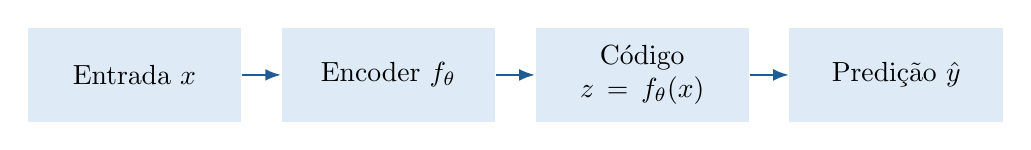
\begin{tikzpicture}
  \node[etapa,text width=25mm] (n0) {Entrada $x$};
  \node[etapa,text width=25mm,right=5mm of n0] (n1) {Encoder $f_\theta$};
  \node[etapa,text width=25mm,right=5mm of n1] (n2) {Código $z=f_\theta(x)$};
  \node[etapa,text width=25mm,right=5mm of n2] (n3) {Predição $\hat{y}$};
  \draw[seta] (n0) -- (n1); \draw[seta] (n1) -- (n2); \draw[seta] (n2) -- (n3);
\end{tikzpicture}\par
\vfill
{\small\color{Suave}O erro em relação ao rótulo ajusta tanto o encoder quanto o preditor.\par}
\vfill
\end{frame}

% Slide 5
\begin{frame}[t]{Utilidade dos rótulos}
\vspace{8mm}
\begin{columns}[onlytextwidth,T]
  \column{.47\textwidth}
  \painel{\linewidth}{Reconhecer o dígito}
  \smallskip
  \begin{itemize}
    \item Indentificação de curvas
    \item Posição dos traços
  \end{itemize}
  \column{.47\textwidth}
  \painel{\linewidth}{Identificar quem escreveu}
  \smallskip
  \begin{itemize}
    \item Largura do traço
    \item Inclinação da escrita
  \end{itemize}
\end{columns}
\vfill
{\centering\large\color{Suave}A utilidade depende da tarefa\par}
\vspace{4mm}
\end{frame}

% Slide 6
\begin{frame}[t]{Pré-treinamento camada por camada}
\vfill
\centering
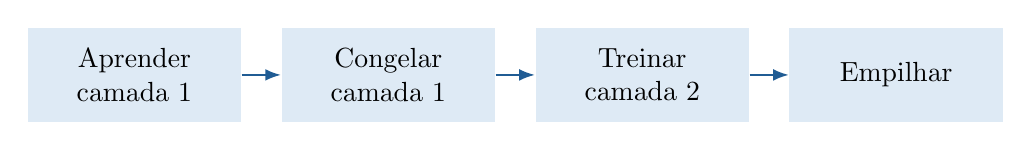
\begin{tikzpicture}
  \node[etapa,text width=25mm] (n0) {Aprender camada 1};
  \node[etapa,text width=25mm,right=5mm of n0] (n1) {Congelar camada 1};
  \node[etapa,text width=25mm,right=5mm of n1] (n2) {Treinar camada 2};
  \node[etapa,text width=25mm,right=5mm of n2] (n3) {Empilhar};
  \draw[seta] (n0) -- (n1);
  \draw[seta] (n1) -- (n2);
  \draw[seta] (n2) -- (n3);
\end{tikzpicture}
\end{frame}

% Slide 7
\begin{frame}[t]{Congelar ou ajustar o encoder}
\smallskip
\begin{columns}[onlytextwidth,T]
  \column{.47\textwidth}
  \painel{\linewidth}{\textbf{Congelar}\\Manter os pesos do encoder}
  \smallskip
  {\small Treina apenas um novo preditor sobre os atributos já aprendidos.\par}
  \smallskip
  {\small\color{Suave}Menor custo.\par}
  \column{.47\textwidth}
  \painel{\linewidth}{\textbf{Fine-tuning}\\Ajustar os pesos do encoder}
  \smallskip
  {\small Adapta a representação à nova tarefa durante o treinamento.\par}
  \smallskip
  {\small\color{Suave}Mais flexível.\par}
\end{columns}
\vfill
{\centering\small A escolha depende dos dados disponíveis e da semelhança entre as tarefas.\par}
\vfill
\end{frame}

% Slide 8
\begin{frame}[t]{O que muda com o pré-treino?}
\smallskip
\begin{columns}[onlytextwidth,T]
  \column{.47\textwidth}
  \painel{\linewidth}{\textbf{Inicialização aleatória}}
  \smallskip
  {\small Os pesos começam sem conhecimento específico; a rede aprende a representação a partir dos dados da tarefa.\par}
  \column{.47\textwidth}
  \painel{\linewidth}{\textbf{Inicialização pré-treinada}}
  \smallskip
  {\small Os pesos começam com padrões aprendidos em dados anteriores e podem ser adaptados à nova tarefa.\par}
\end{columns}
\vfill
{\centering\small\color{Azul}O pré-treino pode acelerar o aprendizado e ajudar quando há poucos rótulos.\par}
\vfill\fonte{Seção 15.1}
\end{frame}

% Slide 9
\begin{frame}[t]{Transferência entre tarefas}
\medskip
Aproveitar conhecimento aprendido em uma tarefa para facilitar outra relacionada.
\vfill
\centering
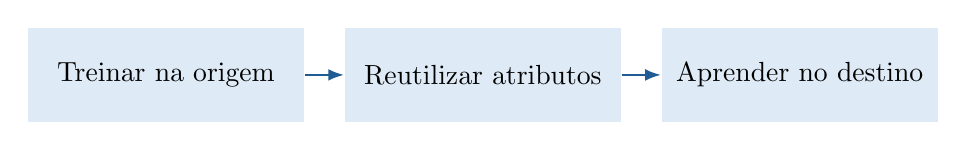
\begin{tikzpicture}
  \node[etapa,text width=33mm] (n0) {Treinar na origem};
  \node[etapa,text width=33mm,right=5mm of n0] (n1) {Reutilizar atributos};
  \node[etapa,text width=33mm,right=5mm of n1] (n2) {Aprender no destino};
  \draw[seta] (n0) -- (n1); \draw[seta] (n1) -- (n2);
\end{tikzpicture}\par
\vfill
{\small\color{Suave}A transferência tende a ser mais útil quando origem e destino compartilham padrões relevantes.\par}
\end{frame}

% Slide 10
\begin{frame}[t]{Adaptação de domínio}
\medskip
\textbf{Problema:} classificar o comentário sobre um produto como positivo ou negativo.
\vfill
\comparar{Avaliações de eletrodomésticos}{Avaliações de produtos de beleza}
\medskip
{\centering\small Outros domínios: livros, eletrônicos e roupas.\par}
\vfill
Treinar com comentários de diferentes categorias ajuda a rede a aprender padrões de sentimento que podem ser reutilizados em um novo domínio, apesar das diferenças de vocabulário.
\end{frame}

% Slide 11
\begin{frame}[t]{Onde compartilhar camadas?}
\medskip
Entradas diferentes podem exigir encoders próprios antes de chegar a uma representação comum.
\vfill
\centering
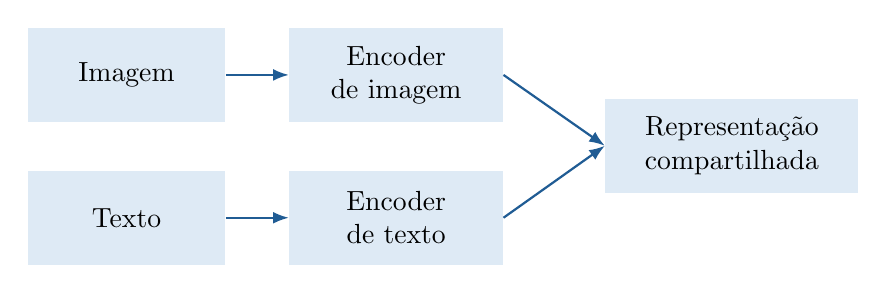
\begin{tikzpicture}[node distance=6mm and 8mm]
  \node[etapa,text width=23mm] (a) {Imagem};
  \node[etapa,text width=25mm,right=of a] (b) {Encoder de imagem};
  \node[etapa,text width=23mm,below=of a] (c) {Texto};
  \node[etapa,text width=25mm,right=of c] (d) {Encoder de texto};
  \node[etapa,text width=30mm] (e) at ([xshift=29mm,yshift=-9mm]b.east) {Representação\\compartilhada};
  \draw[seta] (a) -- (b); \draw[seta] (c) -- (d);
  \draw[seta] (b.east) -- (e.west); \draw[seta] (d.east) -- (e.west);
\end{tikzpicture}\par
\vfill
{\small\color{Suave}Exemplo: aproximar a foto de uma caneca da descrição ``uma caneca''.\par}
\end{frame}

% Slide 12
\begin{frame}[t]{One-shot, zero-shot e a ponte entre modalidades}
\smallskip
\begin{columns}[onlytextwidth,T]
  \column{.47\textwidth}
  \painel{\linewidth}{\textbf{One-shot}\\Um exemplo rotulado por classe}
  \smallskip
  {\small Compara uma nova imagem com o único exemplo disponível de cada classe.\par}
  \smallskip
  {\small\color{Suave}Exemplo: reconhecer uma caneca a partir de uma foto rotulada.\par}
  \column{.47\textwidth}
  \painel{\linewidth}{\textbf{Zero-shot}\\Nenhum exemplo rotulado da classe}
  \smallskip
  {\small Usa conhecimento auxiliar, como uma descrição textual, para reconhecer uma classe não vista no treinamento.\par}
  \smallskip
  {\small\color{Suave}Exemplo: associar uma imagem à descrição ``recipiente com alça''.\par}
\end{columns}
\vfill
{\centering\small\color{Azul}\textbf{Ponte entre modalidades:} imagens e textos podem ser comparados em uma representação compartilhada.\par}
\end{frame}

% Slide 13
\begin{frame}[t]{Fatores de variação}
\vfill
\begin{columns}[onlytextwidth,c]
  \column{.37\textwidth}
  \begin{itemize}
    \item Identidade do objeto
    \medskip
    \item Pose e posição
    \medskip
    \item Iluminação
  \end{itemize}
  \column{.59\textwidth}
  \centering
  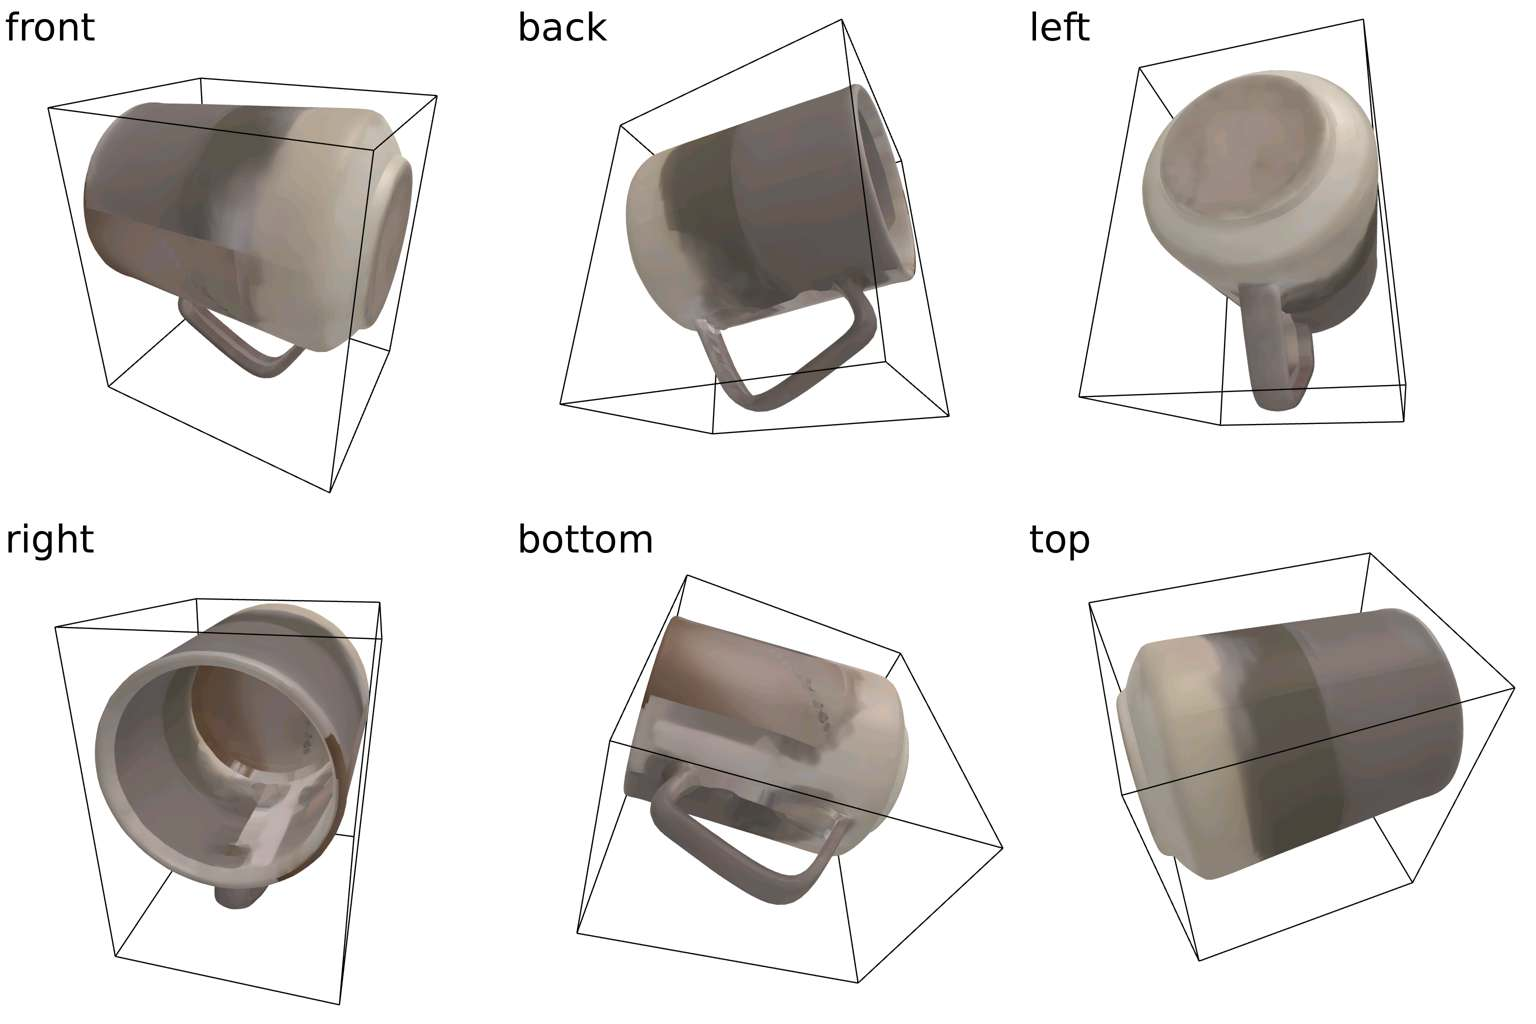
\includegraphics[width=\linewidth,height=46mm,keepaspectratio]{figuras/caneca-angulos.jpg}\par
  {\small A mesma caneca vista de diferentes ângulos.\par}
\end{columns}
\vfill\fonte{Imagem: \href{https://robotwin-platform.github.io/doc/objects/039_mug.html}{RoboTwin 2.0}}
\end{frame}

% Slide 14
\begin{frame}[t]{Quando as entradas dão pistas sobre os rótulos}
\smallskip
\begin{columns}[onlytextwidth,T]
  \column{.47\textwidth}
  \painel{\linewidth}{\textbf{Entradas}\\Distribuição $p(x)$}
  \smallskip
  {\small Mostra como os exemplos se organizam, inclusive os que não têm rótulo.\par}
  \column{.47\textwidth}
  \painel{\linewidth}{\textbf{Rótulos}\\Regra $p(y\mid x)$}
  \smallskip
  {\small Relaciona cada entrada às classes ou saídas que queremos prever.\par}
\end{columns}
\vfill
{\small\textbf{Exemplo:} se imagens de dígitos formam grupos separados, exemplos sem rótulo podem ajudar a identificar a estrutura desses grupos.\par}
\smallskip
{\small\color{Suave}Isso ajuda quando a estrutura das entradas está relacionada às classes; não é garantido em geral.\par}
\vfill\fonte{Seção 15.3}
\end{frame}

% Slide 15
\begin{frame}[t]{O objetivo muda o que se preserva}
\vfill
\centering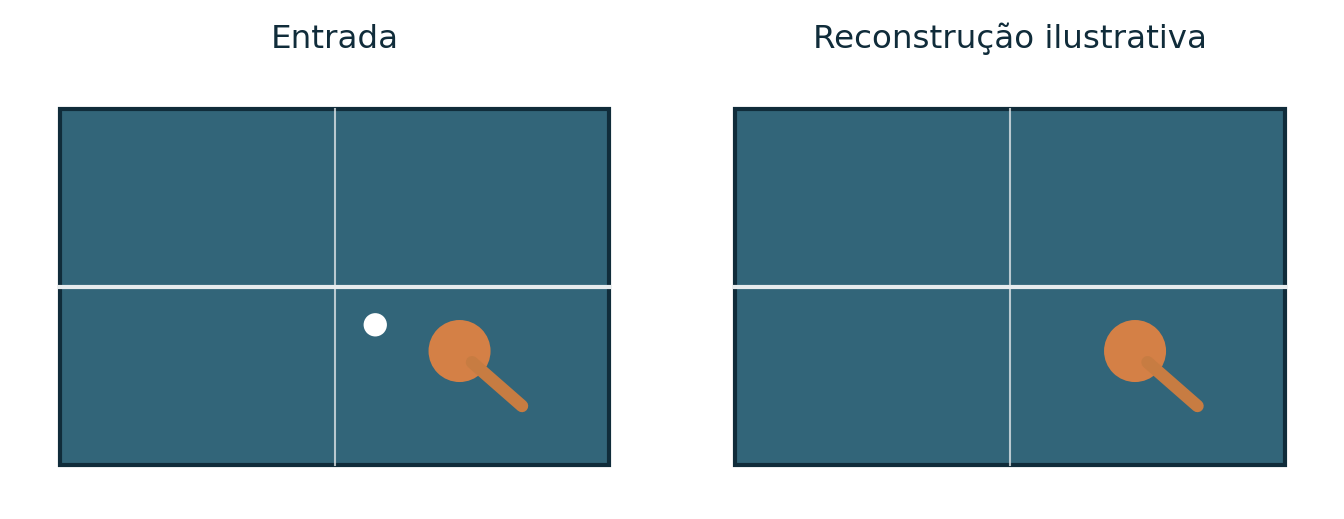
\includegraphics[width=.94\textwidth,height=53mm,keepaspectratio]{figuras/pingue-pongue.png}\par
\fonte{Esquema próprio inspirado na figura 15.5 de Goodfellow et al.}
\end{frame}

% Slide 16
\begin{frame}[t]{Representações distribuídas}
\smallskip
\begin{columns}[onlytextwidth,T]
  \column{.47\textwidth}
  \painel{\linewidth}{\textbf{One-hot}\\Uma posição por categoria}
  \smallskip
  {\small Cada categoria ativa uma posição própria; a representação não explicita atributos compartilhados.\par}
  \column{.47\textwidth}
  \painel{\linewidth}{\textbf{Distribuída}\\Características reutilizadas}
  \smallskip
  {\small Uma categoria é descrita por várias características, que também podem aparecer em outras.\par}
\end{columns}
\vfill
{\small\textbf{Exemplo:} ``círculo vermelho'' e ``quadrado vermelho'' podem compartilhar o atributo \textit{vermelho}.\par}
\vfill\fonte{Seção 15.4}
\end{frame}

% Slide 17
\begin{frame}[t]{Capacidade e restrições geométricas}
\vfill
\centering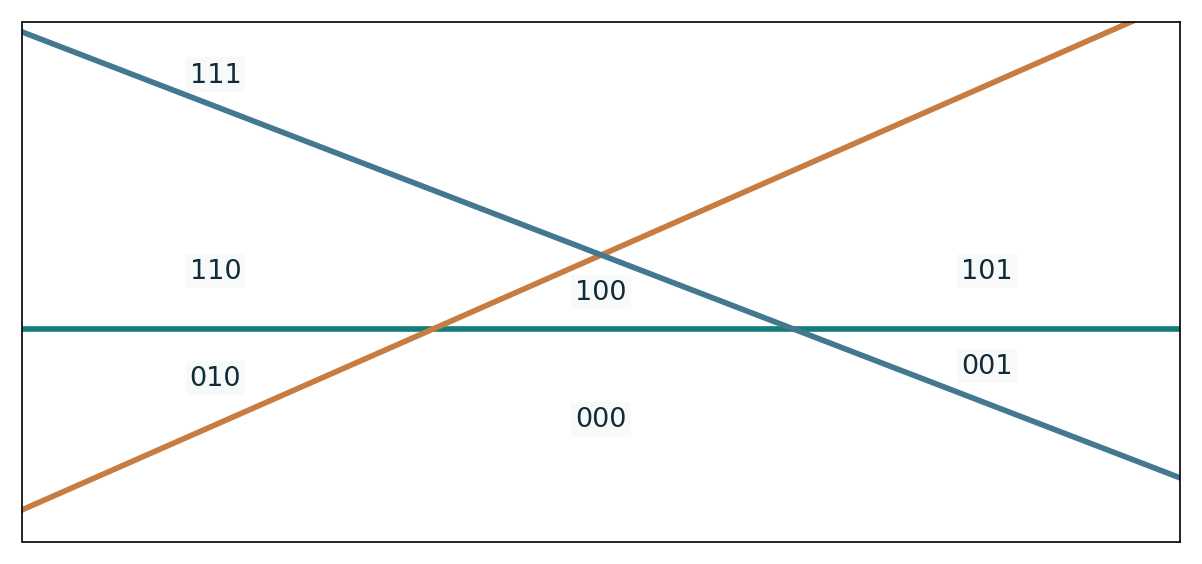
\includegraphics[width=.94\textwidth,height=53mm,keepaspectratio]{figuras/sete-regioes.png}\par
\fonte{Esquema próprio inspirado na figura 15.7 de Goodfellow et al.}
\end{frame}

% Slide 18
\begin{frame}[t]{Generalização por novas combinações}
\medskip
Se a rede aprende separadamente cor e forma, pode reutilizar esses atributos em combinações novas.
\vfill
\centering
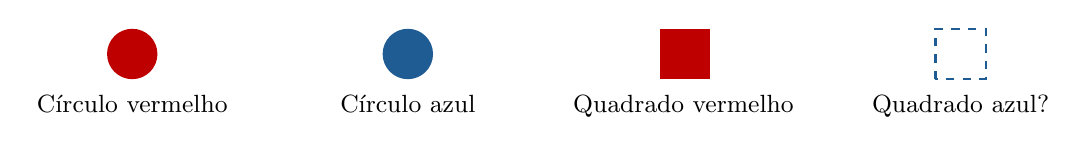
\begin{tikzpicture}[x=1cm,y=1cm]
  \fill[red!75!black] (0,0) circle (.32); \node[below] at (0,-.4) {\small Círculo vermelho};
  \fill[Azul] (3.5,0) circle (.32); \node[below] at (3.5,-.4) {\small Círculo azul};
  \fill[red!75!black] (6.7,-.32) rectangle (7.34,.32); \node[below] at (7,-.4) {\small Quadrado vermelho};
  \draw[Azul,thick,dashed] (10.2,-.32) rectangle (10.84,.32); \node[below] at (10.52,-.4) {\small Quadrado azul?};
\end{tikzpicture}\par
\vfill
{\small\color{Suave}A combinação azul + quadrado não foi apresentada nos exemplos; a generalização depende do que a rede aprendeu.\par}
\end{frame}

% Slide 19
\begin{frame}[t]{Profundidade e composição}
\medskip
Camadas sucessivas podem combinar padrões simples em características mais complexas.
\vfill
\centering
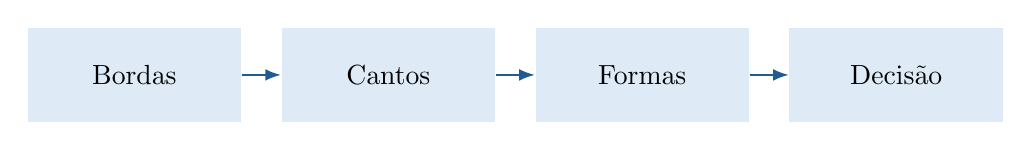
\begin{tikzpicture}
  \node[etapa,text width=25mm] (n0) {Bordas};
  \node[etapa,text width=25mm,right=5mm of n0] (n1) {Cantos};
  \node[etapa,text width=25mm,right=5mm of n1] (n2) {Formas};
  \node[etapa,text width=25mm,right=5mm of n2] (n3) {Decisão};
  \draw[seta] (n0) -- (n1); \draw[seta] (n1) -- (n2); \draw[seta] (n2) -- (n3);
\end{tikzpicture}\par
\vfill
{\small\textbf{Exemplo:} em uma imagem, bordas podem compor contornos; contornos podem ajudar a reconhecer partes de um objeto.\par}
\smallskip
{\small\color{Suave}É uma ilustração conceitual: redes reais não precisam seguir exatamente essa sequência.\par}
\vfill\fonte{Seção 15.5}
\end{frame}

% Slide 20
\begin{frame}[t]{Capacidade, treino e generalização}
\medskip
Três perguntas distintas ajudam a avaliar uma rede:
\vfill
\begin{itemize}
  \item \textbf{Capacidade:} a arquitetura consegue representar a solução desejada?
  \medskip
  \item \textbf{Treinamento:} a otimização encontra parâmetros que resolvem a tarefa?
  \medskip
  \item \textbf{Generalização:} a solução funciona também em exemplos não vistos?
\end{itemize}
\vfill
{\small\color{Suave}Exemplo: memorizar as imagens de treino não garante reconhecer novos dígitos.\par}
\end{frame}

% Slide 21
\begin{frame}[t]{Pistas sobre os dados}
\medskip
Hipóteses sobre a estrutura dos dados orientam a construção de representações:
\vfill
\begin{itemize}
  \item \textbf{Suavidade local:} pequenas mudanças na entrada tendem a preservar a saída.
  \medskip
  \item \textbf{Fatores e hierarquia:} características podem variar separadamente e se combinar em padrões mais complexos.
  \medskip
  \item \textbf{Compartilhamento e grupos:} exemplos podem reutilizar atributos e formar agrupamentos.
\end{itemize}
\vfill
{\small\color{Suave}Exemplo: imagens de uma caneca podem variar em posição e iluminação mantendo sua identidade.\par}
\vfill\fonte{Seção 15.6}
\end{frame}

% Slide 22
\begin{frame}[t]{Espaço, tempo e esparsidade}
\medskip
Outras hipóteses podem ajudar a encontrar estruturas úteis nos dados:
\vfill
\begin{itemize}
  \item \textbf{Coerência espacial:} pixels próximos frequentemente descrevem partes relacionadas de uma imagem.
  \medskip
  \item \textbf{Coerência temporal:} quadros próximos de um vídeo tendem a mudar gradualmente.
  \medskip
  \item \textbf{Esparsidade:} apenas parte das características pode ser necessária para descrever cada exemplo.
\end{itemize}
\vfill
{\small\color{Suave}Exemplo: em um vídeo de uma caneca, sua posição muda entre quadros, mas sua identidade tende a permanecer.\par}
\vfill\fonte{Seção 15.6}
\end{frame}

% Slide 23
\begin{frame}[t]{O que um leitor simples extrai do código?}
\vfill
\centering
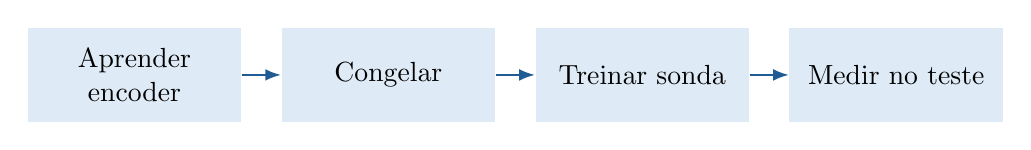
\begin{tikzpicture}
  \node[etapa,text width=25mm] (n0) {Aprender encoder};
  \node[etapa,text width=25mm,right=5mm of n0] (n1) {Congelar};
  \node[etapa,text width=25mm,right=5mm of n1] (n2) {Treinar sonda};
  \node[etapa,text width=25mm,right=5mm of n2] (n3) {Medir no teste};
  \draw[seta] (n0) -- (n1);
  \draw[seta] (n1) -- (n2);
  \draw[seta] (n2) -- (n3);
\end{tikzpicture}\par
\vfill\fonte{Avaliação}
\end{frame}

% Slide 24
\begin{frame}[t]{Mesmas entradas, duas tarefas}
\vfill
\centering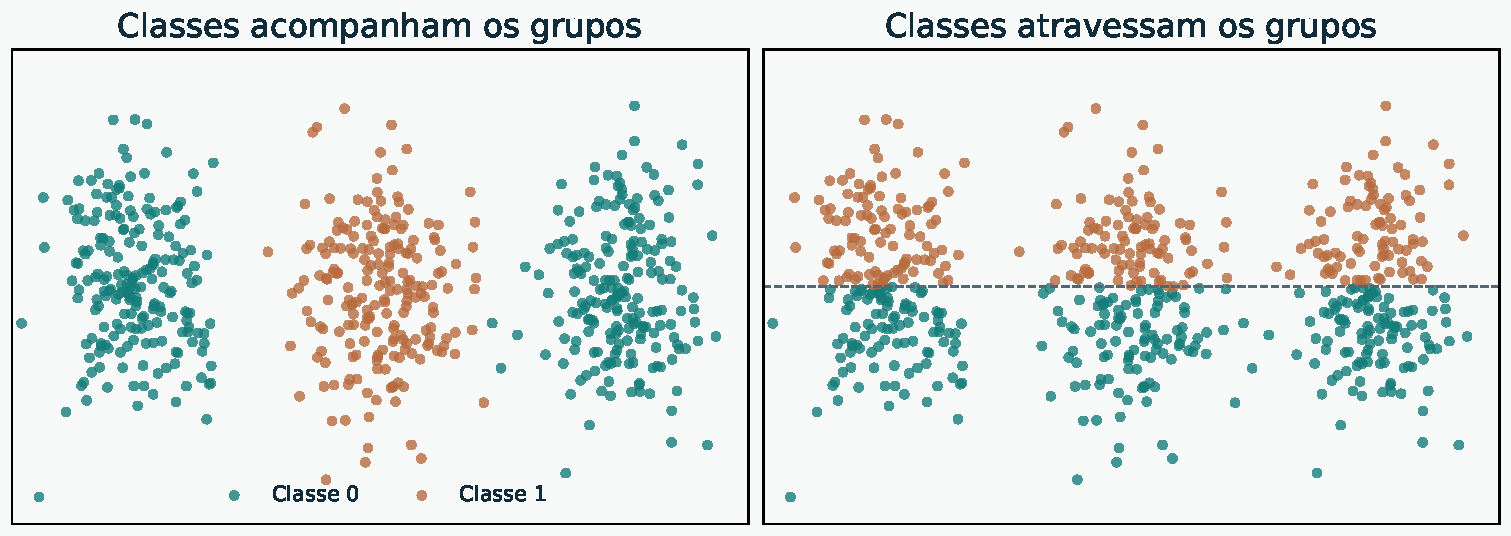
\includegraphics[width=.94\textwidth,height=53mm,keepaspectratio]{figuras/grupos.pdf}\par
\fonte{Dados sintéticos. As cores mostram os rótulos das duas tarefas.}
\vfill\fonte{Seção 15.3}
\end{frame}

% Slide 25
\begin{frame}[t]{Quando agrupar ajuda}
\vfill
\centering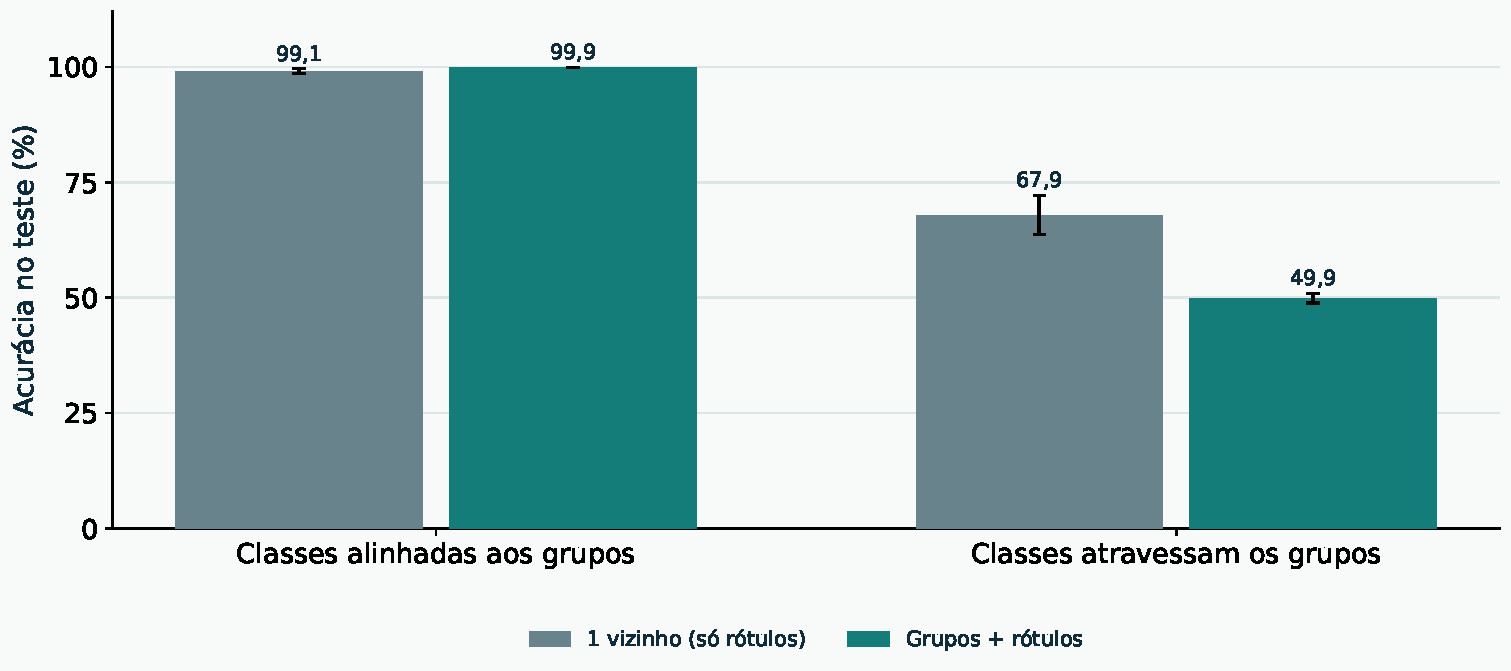
\includegraphics[width=.94\textwidth,height=53mm,keepaspectratio]{figuras/resultado-grupos.pdf}\par
\fonte{Teste independente. Média e desvio padrão de cinco sorteios.}
\end{frame}

% Slide 26
\begin{frame}[t]{Transferência para dígitos novos}
\vfill
\begin{itemize}
  \item Origem: classes de 0 a 4
  \medskip
  \item Destino: classes de 5 a 9
  \medskip
  \item Rótulos: 5 ou 20 por classe
\end{itemize}
\centering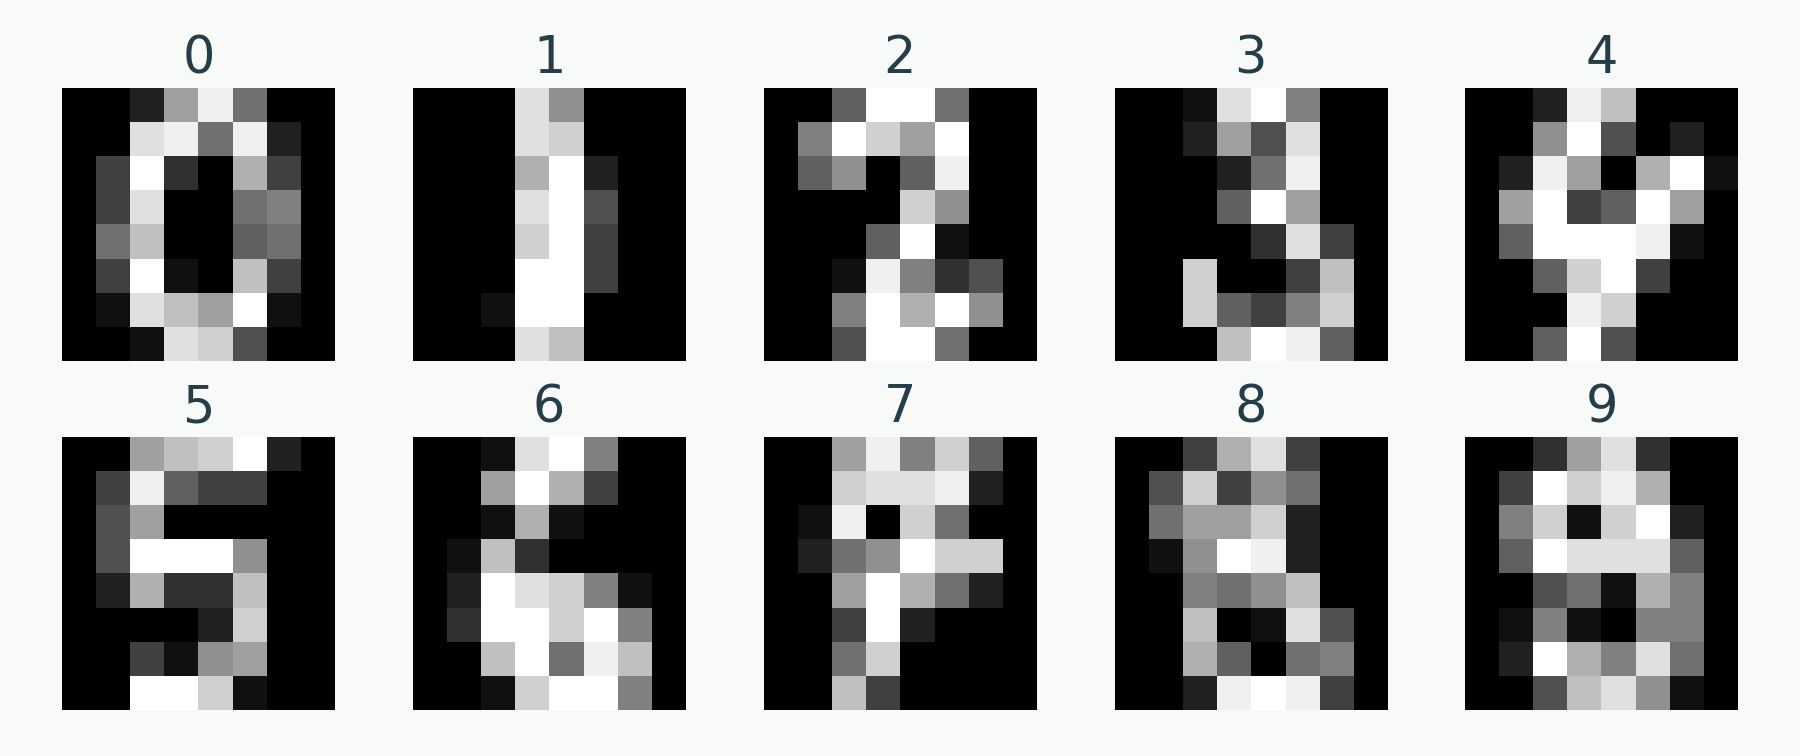
\includegraphics[height=21mm]{figuras/digits.png}\par
\end{frame}

% Slide 27
\begin{frame}[t]{O pré-treino ajudou em relação ao quê?}
\vfill
\centering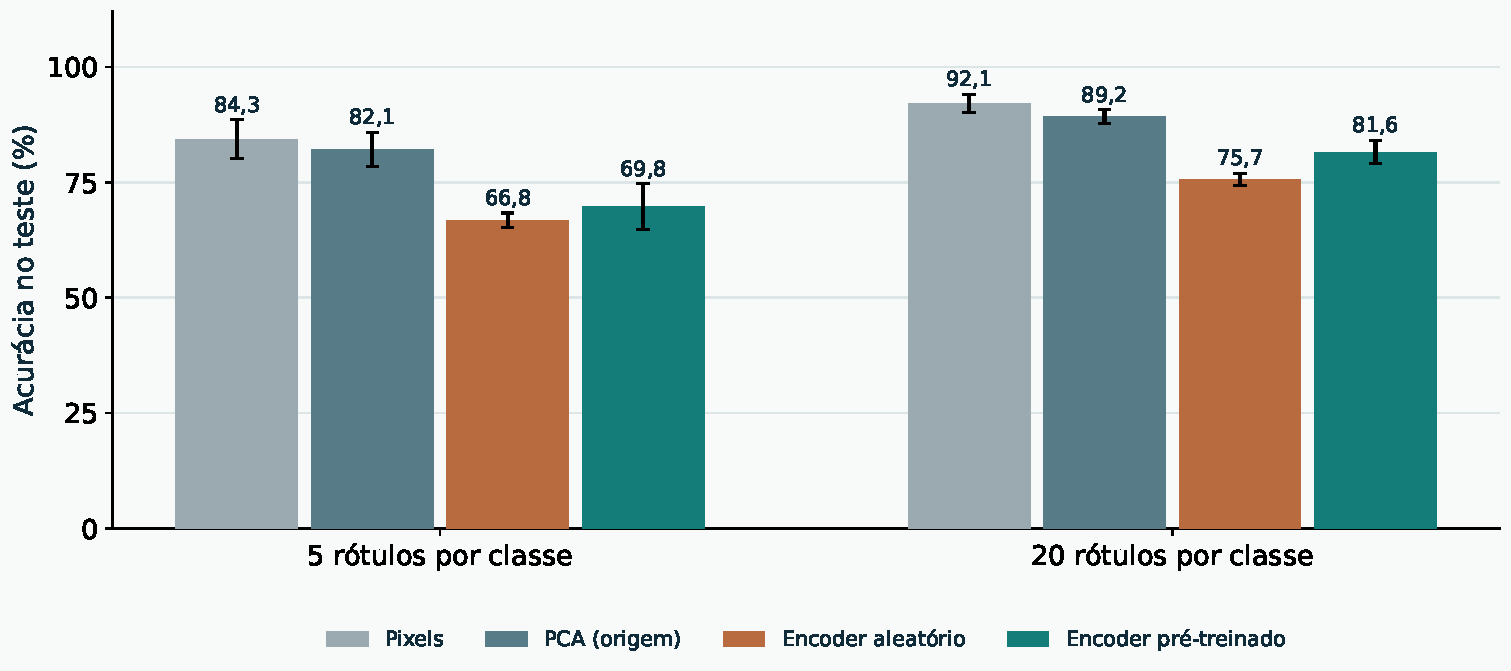
\includegraphics[width=.94\textwidth,height=53mm,keepaspectratio]{figuras/resultado-transferencia.pdf}\par
\fonte{Teste nos dígitos 5 a 9. Média e desvio padrão de cinco execuções.}
\end{frame}

% Slide 28
\begin{frame}[t]{Representações em aplicações práticas}
\vfill
\begin{itemize}
  \item Inspeção visual: detectar e localizar defeitos
  \medskip
  \item Sensores: transferir entre condições de aquisição
  \medskip
  \item Pesquisa: recuperar imagens semelhantes
\end{itemize}
\vfill\fonte{Aplicações possíveis}
\end{frame}

% Slide 29
\begin{frame}[t]{Inovação: classificar com descrições}
\vfill
\centering
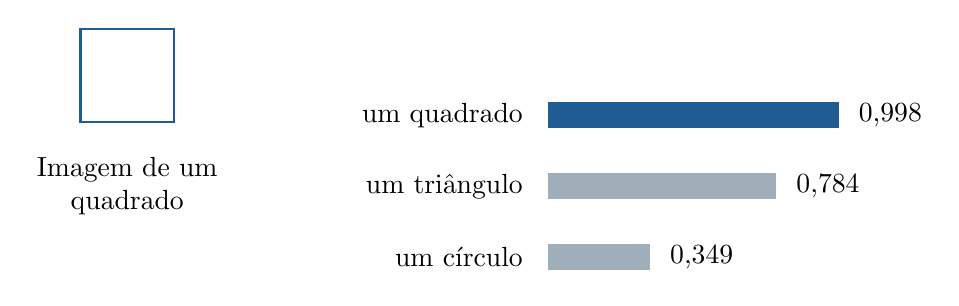
\begin{tikzpicture}[x=66mm,y=9mm]
  \node[align=center] at (-.38,-1) {Imagem de um\\quadrado};
  \draw[thick,Azul] (-.47,-.10) rectangle (-.29,1.22);
  \node[anchor=east] at (.40,0) {um quadrado};
  \fill[Azul] (.43,-0.18) rectangle (0.989,0.18);
  \node[anchor=west] at (1.009,0) {0,998};
  \node[anchor=east] at (.40,-1) {um triângulo};
  \fill[Suave!55] (.43,-1.18) rectangle (0.869,-0.82);
  \node[anchor=west] at (0.889,-1) {0,784};
  \node[anchor=east] at (.40,-2) {um círculo};
  \fill[Suave!55] (.43,-2.18) rectangle (0.626,-1.82);
  \node[anchor=west] at (0.646,-2) {0,349};
\end{tikzpicture}\par
\fonte{Similaridade de cosseno. Exemplo com vetores sintéticos.}
\vfill\fonte{Radford et al. (2021)}
\end{frame}

% Slide 30
\begin{frame}[t]{Inovação: características com posição}
\vfill
\centering
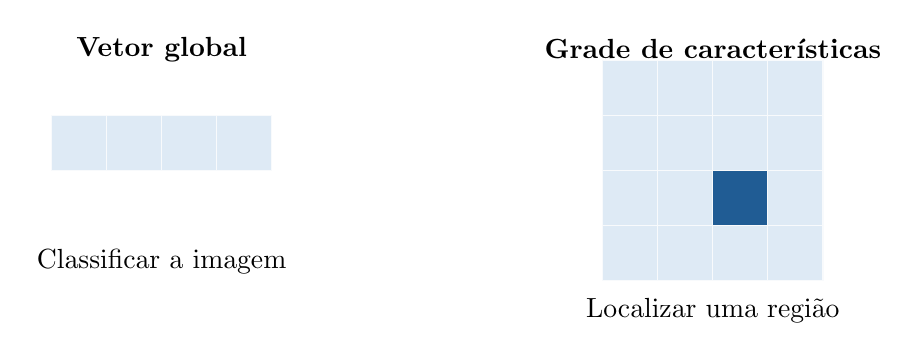
\begin{tikzpicture}[x=7mm,y=7mm]
  \node[font=\bfseries] at (2,4.2) {Vetor global};
  \node[font=\bfseries] at (12,4.2) {Grade de características};
  \foreach \x in {0,1,2,3} {
    \filldraw[fill=Claro,draw=Fundo] (\x,2) rectangle ++(1,1);
  }
  \foreach \x in {10,11,12,13} {
    \foreach \y in {0,1,2,3} {
      \filldraw[fill=Claro,draw=Fundo] (\x,\y) rectangle ++(1,1);
    }
  }
  \filldraw[fill=Azul,draw=Fundo] (12,1) rectangle ++(1,1);
  \node at (2,.35) {Classificar a imagem};
  \node at (12,-.55) {Localizar uma região};
\end{tikzpicture}\par
\fonte{Esquema conceitual inspirado no uso de características densas.}
\vfill\fonte{Siméoni et al. (2025)}
\end{frame}

% Slide 31
\begin{frame}[t]{Objetivo, representação e tarefa}
\vfill
\centering
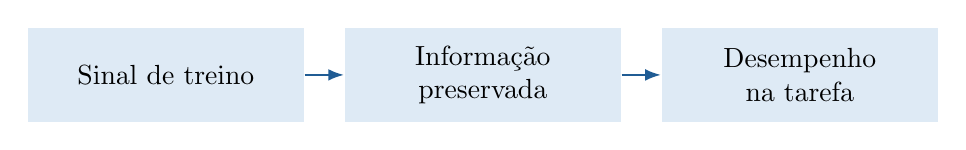
\begin{tikzpicture}
  \node[etapa,text width=33mm] (n0) {Sinal de treino};
  \node[etapa,text width=33mm,right=5mm of n0] (n1) {Informação preservada};
  \node[etapa,text width=33mm,right=5mm of n1] (n2) {Desempenho na tarefa};
  \draw[seta] (n0) -- (n1);
  \draw[seta] (n1) -- (n2);
\end{tikzpicture}\par
\end{frame}

% Slide 32
{
\setbeamercolor{background canvas}{bg=Tinta}
\setbeamercolor{normal text}{fg=white,bg=Tinta}
\setbeamertemplate{background}{%
  \begin{tikzpicture}[remember picture,overlay]
    \fill[white] ([xshift=-.55\paperwidth]current page.north east) -- (current page.north east) -- ([yshift=-.48\paperheight]current page.north east) -- cycle;
    \node[anchor=north east,inner sep=0pt] at ([xshift=-6mm,yshift=-4mm]current page.north east) {
\includegraphics[width=36mm]{figuras/lps.png}};
  \end{tikzpicture}%
}
\begin{frame}[plain]
  \color{white}
  \vfill
  {\huge\bfseries Obrigado!\par}
  \vfill
\end{frame}
}

\end{document}
